\documentclass[11pt, fleqn]{article}

\usepackage{amsmath}
\usepackage{amssymb}
\usepackage[linesnumbered,ruled,vlined]{algorithm2e}
\usepackage{amsthm}
\usepackage{mathtools}
\usepackage{hyperref}
\usepackage{ulem}
\usepackage{enumitem}
\usepackage[left=0.75in, right=0.75in, bottom=0.75in, top=1.0in]{geometry}
\usepackage{floatrow}
\usepackage{float}
\usepackage{graphicx}
\usepackage[export]{adjustbox}
\usepackage{sectsty}
\sectionfont{\centering}
\usepackage{hyperref}
\usepackage[dvipsnames]{xcolor}
\usepackage[perpage]{footmisc}

\usepackage{wrapfig}
\usepackage{lscape}
\usepackage{rotating}

\usepackage{fancyhdr}
\pagestyle{fancy}
\fancyhf{}
\lhead{190050020 \& 190100044 \& 190100055 \& 190260036}
\rhead{CS 226: Course Project}
\renewcommand{\footrulewidth}{1.0pt}
\cfoot{Page \thepage}

\SetKwInput{KwInput}{Input}                % Set the Input
\SetKwInput{KwOutput}{Output}              % set the Output
\DeclarePairedDelimiter\ceil{\lceil}{\rceil}
\DeclarePairedDelimiter\floor{\lfloor}{\rfloor}
\newtheorem{lemma}{Lemma}

\newcommand{\boxedeq}[2]{\begin{empheq}[box={\fboxsep=6pt\fbox}]{align}\label{#1}#2\end{empheq}}
\setlength{\parindent}{0em}
\renewcommand{\arraystretch}{2}

\title{CS 226: Course Project}
\author{
\begin{tabular}{|c|c|c|c|}
     \hline
     Ankit Kumar Misra & Devansh Jain & Harshit Varma & Richeek Das \\
     \hline
     190050020 & 190100044 & 190100055 & 190260036\\
     \hline
\end{tabular}
}

\date{\today}

\begin{document}

\maketitle
\tableofcontents
\thispagestyle{empty}
\setcounter{page}{0}
\renewcommand{\arraystretch}{1}

\newpage
\section*{Data Paths}
\addcontentsline{toc}{section}{Data Paths}

\subsection*{\centering Si}
\begin{figure}[H]
    \centering
    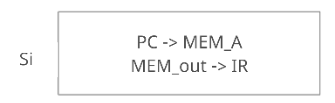
\includegraphics{DataPath/DataPath_Si.PNG}
\end{figure}
\begin{center}
\textbf{Control pins}: \\
Register IR write \\
MUX 2 select 01 \\
\end{center}

\bigskip

\subsection*{\centering S0}
\begin{figure}[H]
    \centering
    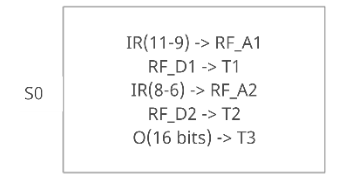
\includegraphics{DataPath/DataPath_S0.PNG}
\end{figure}
\begin{center}
\textbf{Control pins}: \\
Register T1 write \\
Register T2 write \\
Register T3 write \\
MUX 6 select 0 \\
MUX 7 select 01 \\
MUX 8 select 01 \\
\end{center}

\bigskip

\subsection*{\centering S1A}
\begin{figure}[H]
    \centering
    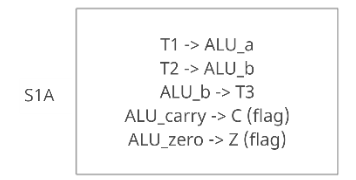
\includegraphics{DataPath/DataPath_S1A.PNG}
\end{figure}
\begin{center}
\textbf{Control pins}: \\
Register T3 write \\
MUX 8 select 10 \\
MUX 9 select 10 \\
MUX 10 select 10 \\
if (op\_code is "0000") then alu\_control is 0, carry write, zero write \\
else alu\_control is 1, zero write \\
\end{center}

\bigskip

\subsection*{\centering S1B}
\begin{figure}[H]
    \centering
    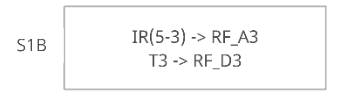
\includegraphics{DataPath/DataPath_S1B.PNG}
\end{figure}
\begin{center}
\textbf{Control pins}: \\
Register RF write \\
MUX 4 select 10 \\
MUX 5 select 11 \\
\end{center}

\bigskip

\subsection*{\centering S2A}
\begin{figure}[H]
    \centering
    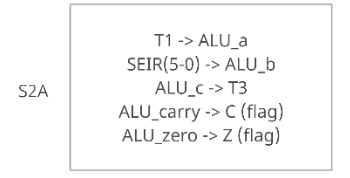
\includegraphics{DataPath/DataPath_S2A.PNG}
\end{figure}
\begin{center}
\textbf{Control pins}: \\
Register T3 write \\
MUX 6 select 10 \\
MUX 9 select 01 \\
MUX 10 select 10 \\
carry write, zero write \\
\end{center}

\bigskip

\subsection*{\centering S2B}
\begin{figure}[H]
    \centering
    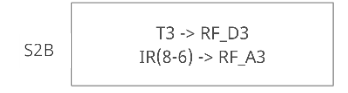
\includegraphics{DataPath/DataPath_S2B.PNG}
\end{figure}
\begin{center}
\textbf{Control pins}: \\
Register RF write \\
MUX 4 select 10 \\
MUX 5 select 11 \\
\end{center}

\bigskip

\subsection*{\centering S3}
\begin{figure}[H]
    \centering
    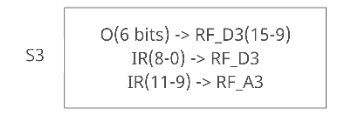
\includegraphics{DataPath/DataPath_S3.PNG}
\end{figure}
\begin{center}
\textbf{Control pins}: \\
Register RF write \\
MUX 4 select 00 \\
MUX 5 select 01 \\
\end{center}

\bigskip

\subsection*{\centering S4}
\begin{figure}[H]
    \centering
    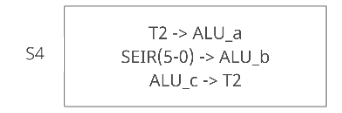
\includegraphics{DataPath/DataPath_S4.PNG}
\end{figure}
\begin{center}
\textbf{Control pins}: \\
Register T2 write \\
MUX 7 select 10 \\
MUX 9 select 01 \\
MUX 10 select 11 \\
\end{center}

\bigskip

\subsection*{\centering S5A}
\begin{figure}[H]
    \centering
    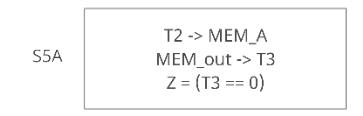
\includegraphics{DataPath/DataPath_S5A.PNG}
\end{figure}
\begin{center}
\textbf{Control pins}: \\
Register T3 write \\
MUX 2 select 00 \\
MUX 8 select 00 \\
MUX 11 select 1 \\
zero write \\
\end{center}

\bigskip

\subsection*{\centering S5B}
\begin{figure}[H]
    \centering
    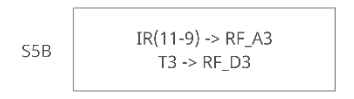
\includegraphics{DataPath/DataPath_S5B.PNG}
\end{figure}
\begin{center}
\textbf{Control pins}: \\
Register RF write \\
MUX 4 select 00 \\
MUX 5 select 11 \\
\end{center}

\bigskip

\subsection*{\centering S6}
\begin{figure}[H]
    \centering
    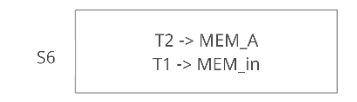
\includegraphics{DataPath/DataPath_S6.PNG}
\end{figure}
\begin{center}
\textbf{Control pins}: \\
Register MEM write \\
MUX 2 select 00 \\
\end{center}

\bigskip

\subsection*{\centering S7A}
\begin{figure}[H]
    \centering
    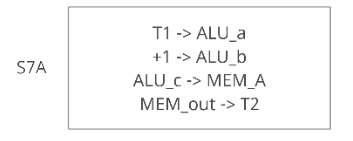
\includegraphics{DataPath/DataPath_S7A.PNG}
\end{figure}
\begin{center}
\textbf{Control pins}: \\
Register T1 write \\
Register T2 write \\
MUX 2 select 11 \\
MUX 6 select 1 \\
MUX 7 select 11 \\
MUX 9 select 11 \\
MUX 10 select 01 \\
\end{center}

\bigskip

\subsection*{\centering S7B}
\begin{figure}[H]
    \centering
    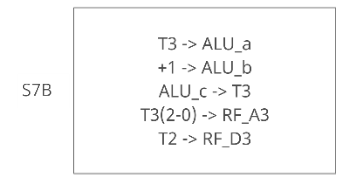
\includegraphics{DataPath/DataPath_S7B.PNG}
\end{figure}
\begin{center}
\textbf{Control pins}: \\
Register RF write \\
Register T3 write \\
MUX 4 select 11 \\
MUX 5 select 10 \\
MUX 8 select 10 \\
MUX 9 select 11 \\
MUX 10 select 00 \\
\end{center}

\bigskip

\subsection*{\centering S8A}
\begin{figure}[H]
    \centering
    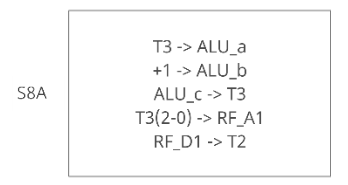
\includegraphics{DataPath/DataPath_S8A.PNG}
\end{figure}
\begin{center}
\textbf{Control pins}: \\
Register T2 write \\
Register T3 write \\
MUX 3 select 1 \\
MUX 7 select 00 \\
MUX 8 select 10 \\
MUX 9 select 11 \\
MUX 10 select 00 \\
\end{center}

\bigskip

\subsection*{\centering S8B}
\begin{figure}[H]
    \centering
    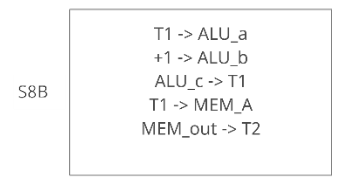
\includegraphics{DataPath/DataPath_S8B.PNG}
\end{figure}
\begin{center}
\textbf{Control pins}: \\
Register MEM write \\
Register T1 write \\
MUX 2 select 11 \\
MUX 6 select 1 \\
MUX 9 select 11 \\
MUX 10 select 10 \\
MUX 12 select 1 \\
\end{center}

\bigskip

\subsection*{\centering S9}
\begin{figure}[H]
    \centering
    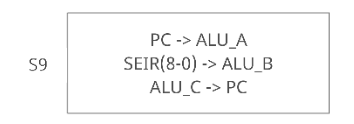
\includegraphics{DataPath/DataPath_S9.PNG}
\end{figure}
\begin{center}
\textbf{Control pins}: \\
Register PC write \\
MUX 1 select 0 \\
MUX 9 select 01 \\
MUX 10 select 01 \\
\end{center}

\bigskip

\subsection*{\centering S10}
\begin{figure}[H]
    \centering
    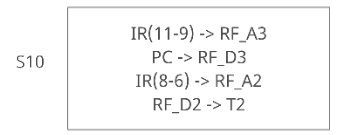
\includegraphics{DataPath/DataPath_S10.PNG}
\end{figure}
\begin{center}
\textbf{Control pins}: \\
Register RF write \\
Register T2 write \\
MUX 4 select 00 \\
MUX 5 select 00 \\
MUX 7 select 01 \\
\end{center}

\bigskip

\subsection*{\centering S11}
\begin{figure}[H]
    \centering
    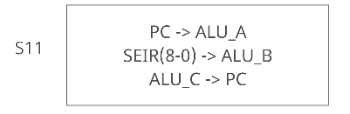
\includegraphics{DataPath/DataPath_S11.PNG}
\end{figure}
\begin{center}
\textbf{Control pins}: \\
Register PC write \\
MUX 1 select 0 \\
MUX 9 select 00 \\
MUX 10 select 01 \\
\end{center}

\bigskip

\subsection*{\centering S12}
\begin{figure}[H]
    \centering
    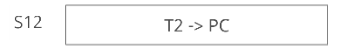
\includegraphics{DataPath/DataPath_S12.PNG}
\end{figure}
\begin{center}
\textbf{Control pins}: \\
Register PC write \\
MUX 1 select 1 \\
\end{center}

\bigskip

\subsection*{\centering Sf}
\begin{figure}[H]
    \centering
    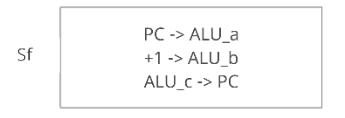
\includegraphics{DataPath/DataPath_Sf.PNG}
\end{figure}
\begin{center}
\textbf{Control pins}: \\
Register PC write \\
MUX 1 select 0 \\
MUX 9 select 11 \\
MUX 10 select 01 \\
\end{center}

\newpage
\section*{State Transition Diagram}
\addcontentsline{toc}{section}{State Transition Diagram}
\begin{figure}[H]
    \centering
    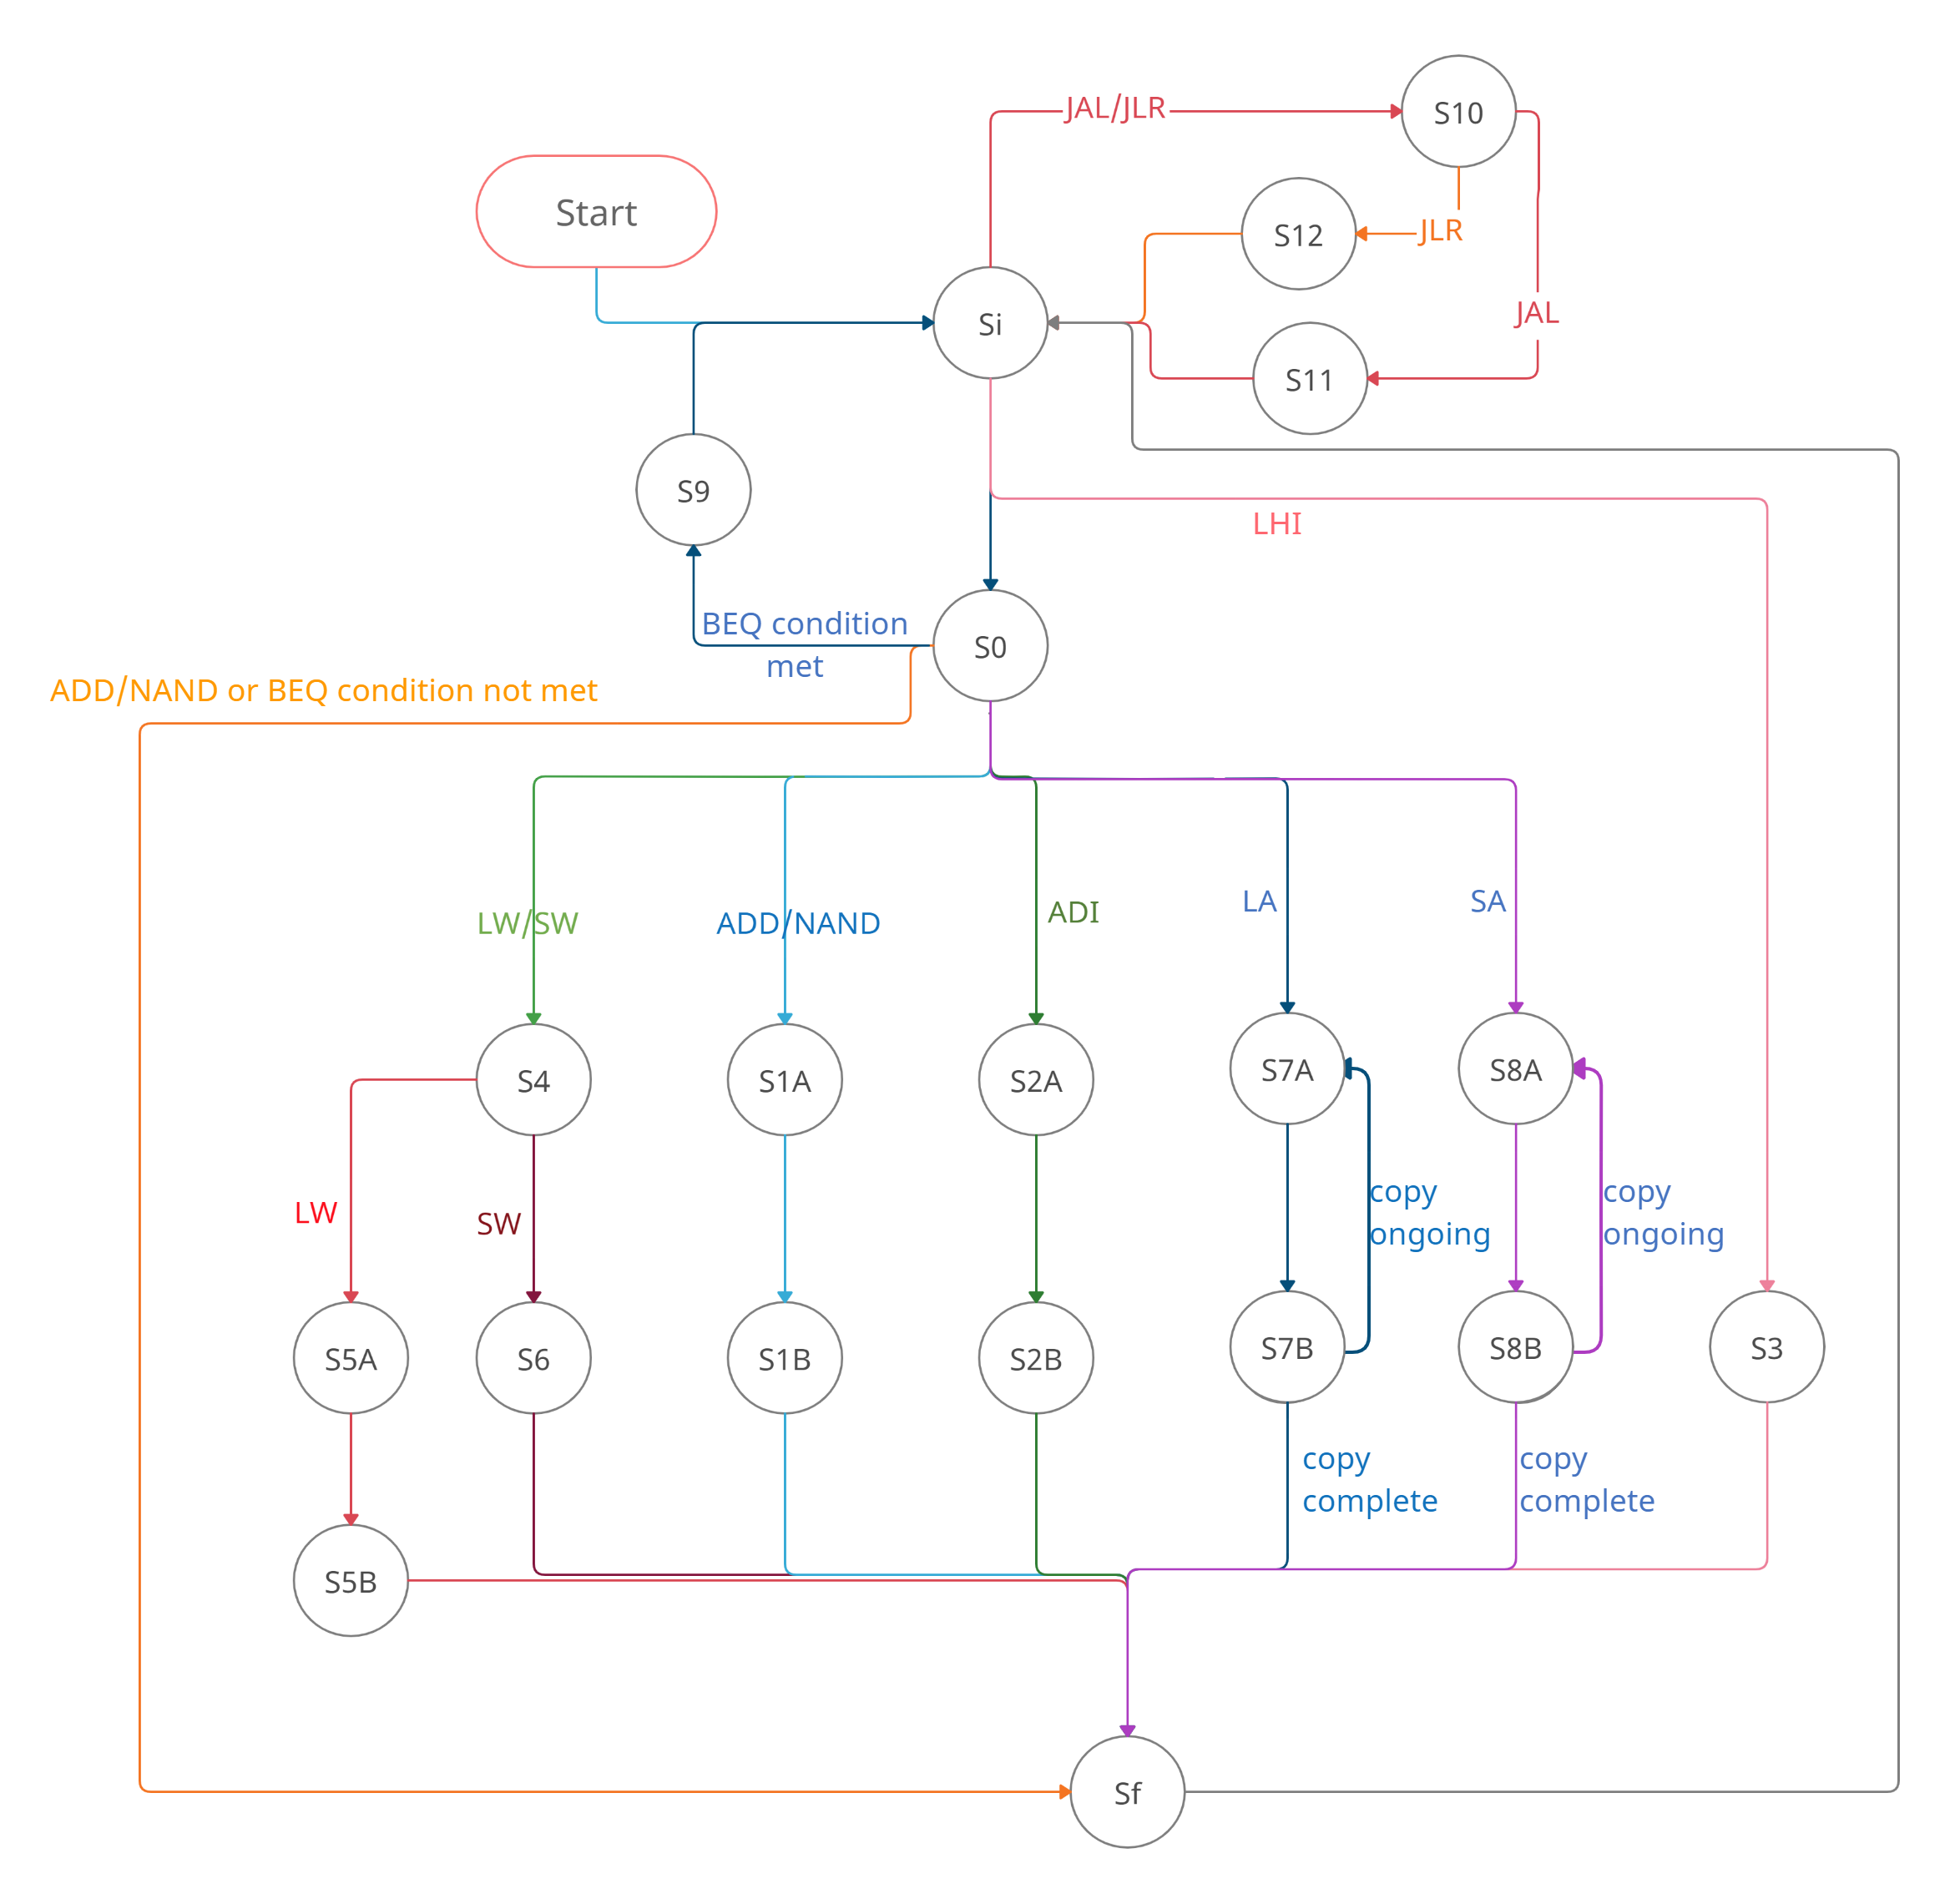
\includegraphics[scale=0.2]{STG.png}
\end{figure}

\newpage
\section*{Circuit Diagram}%
\addcontentsline{toc}{section}{Circuit Diagram}
\vspace*{-0.5cm}
\begin{sidewaysfigure}[H]
    \centering
    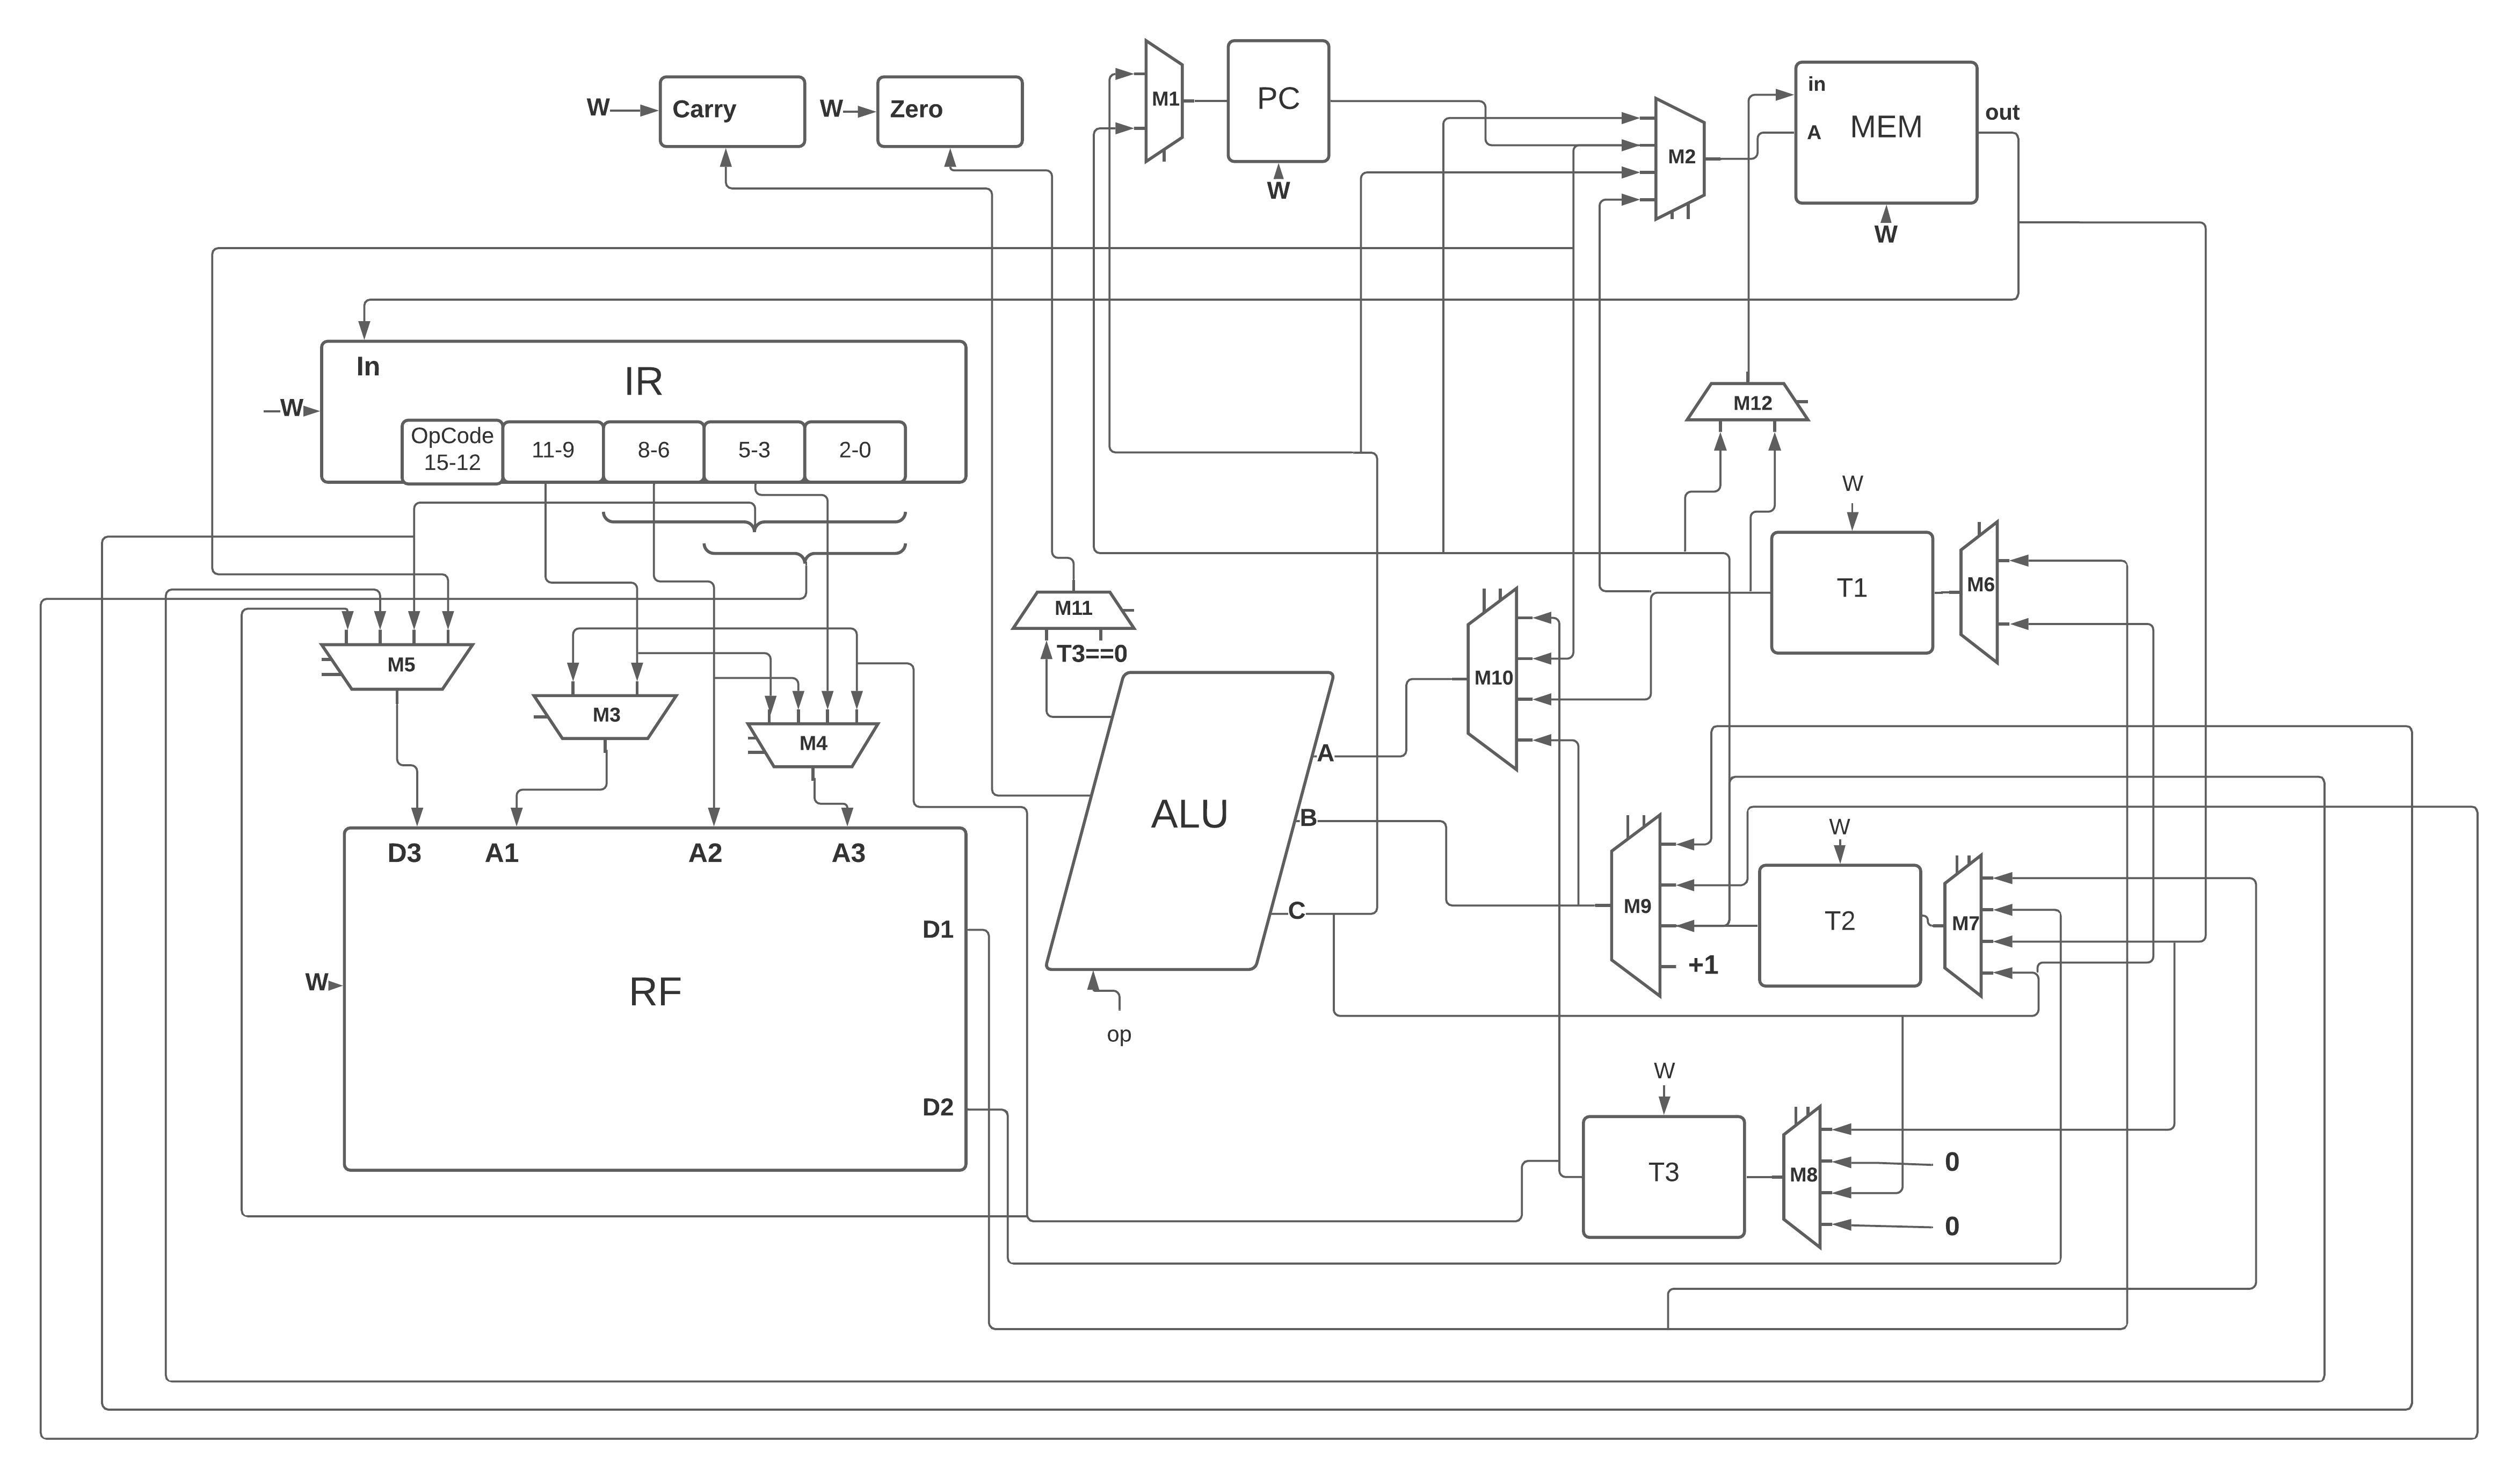
\includegraphics[scale=0.58]{crd.jpeg}
\end{sidewaysfigure}

\newpage
\section*{State Machine Viewer}
\addcontentsline{toc}{section}{State Machine Viewer}
\vspace*{-0.5cm}
\begin{sidewaysfigure}[H]
    \centering
    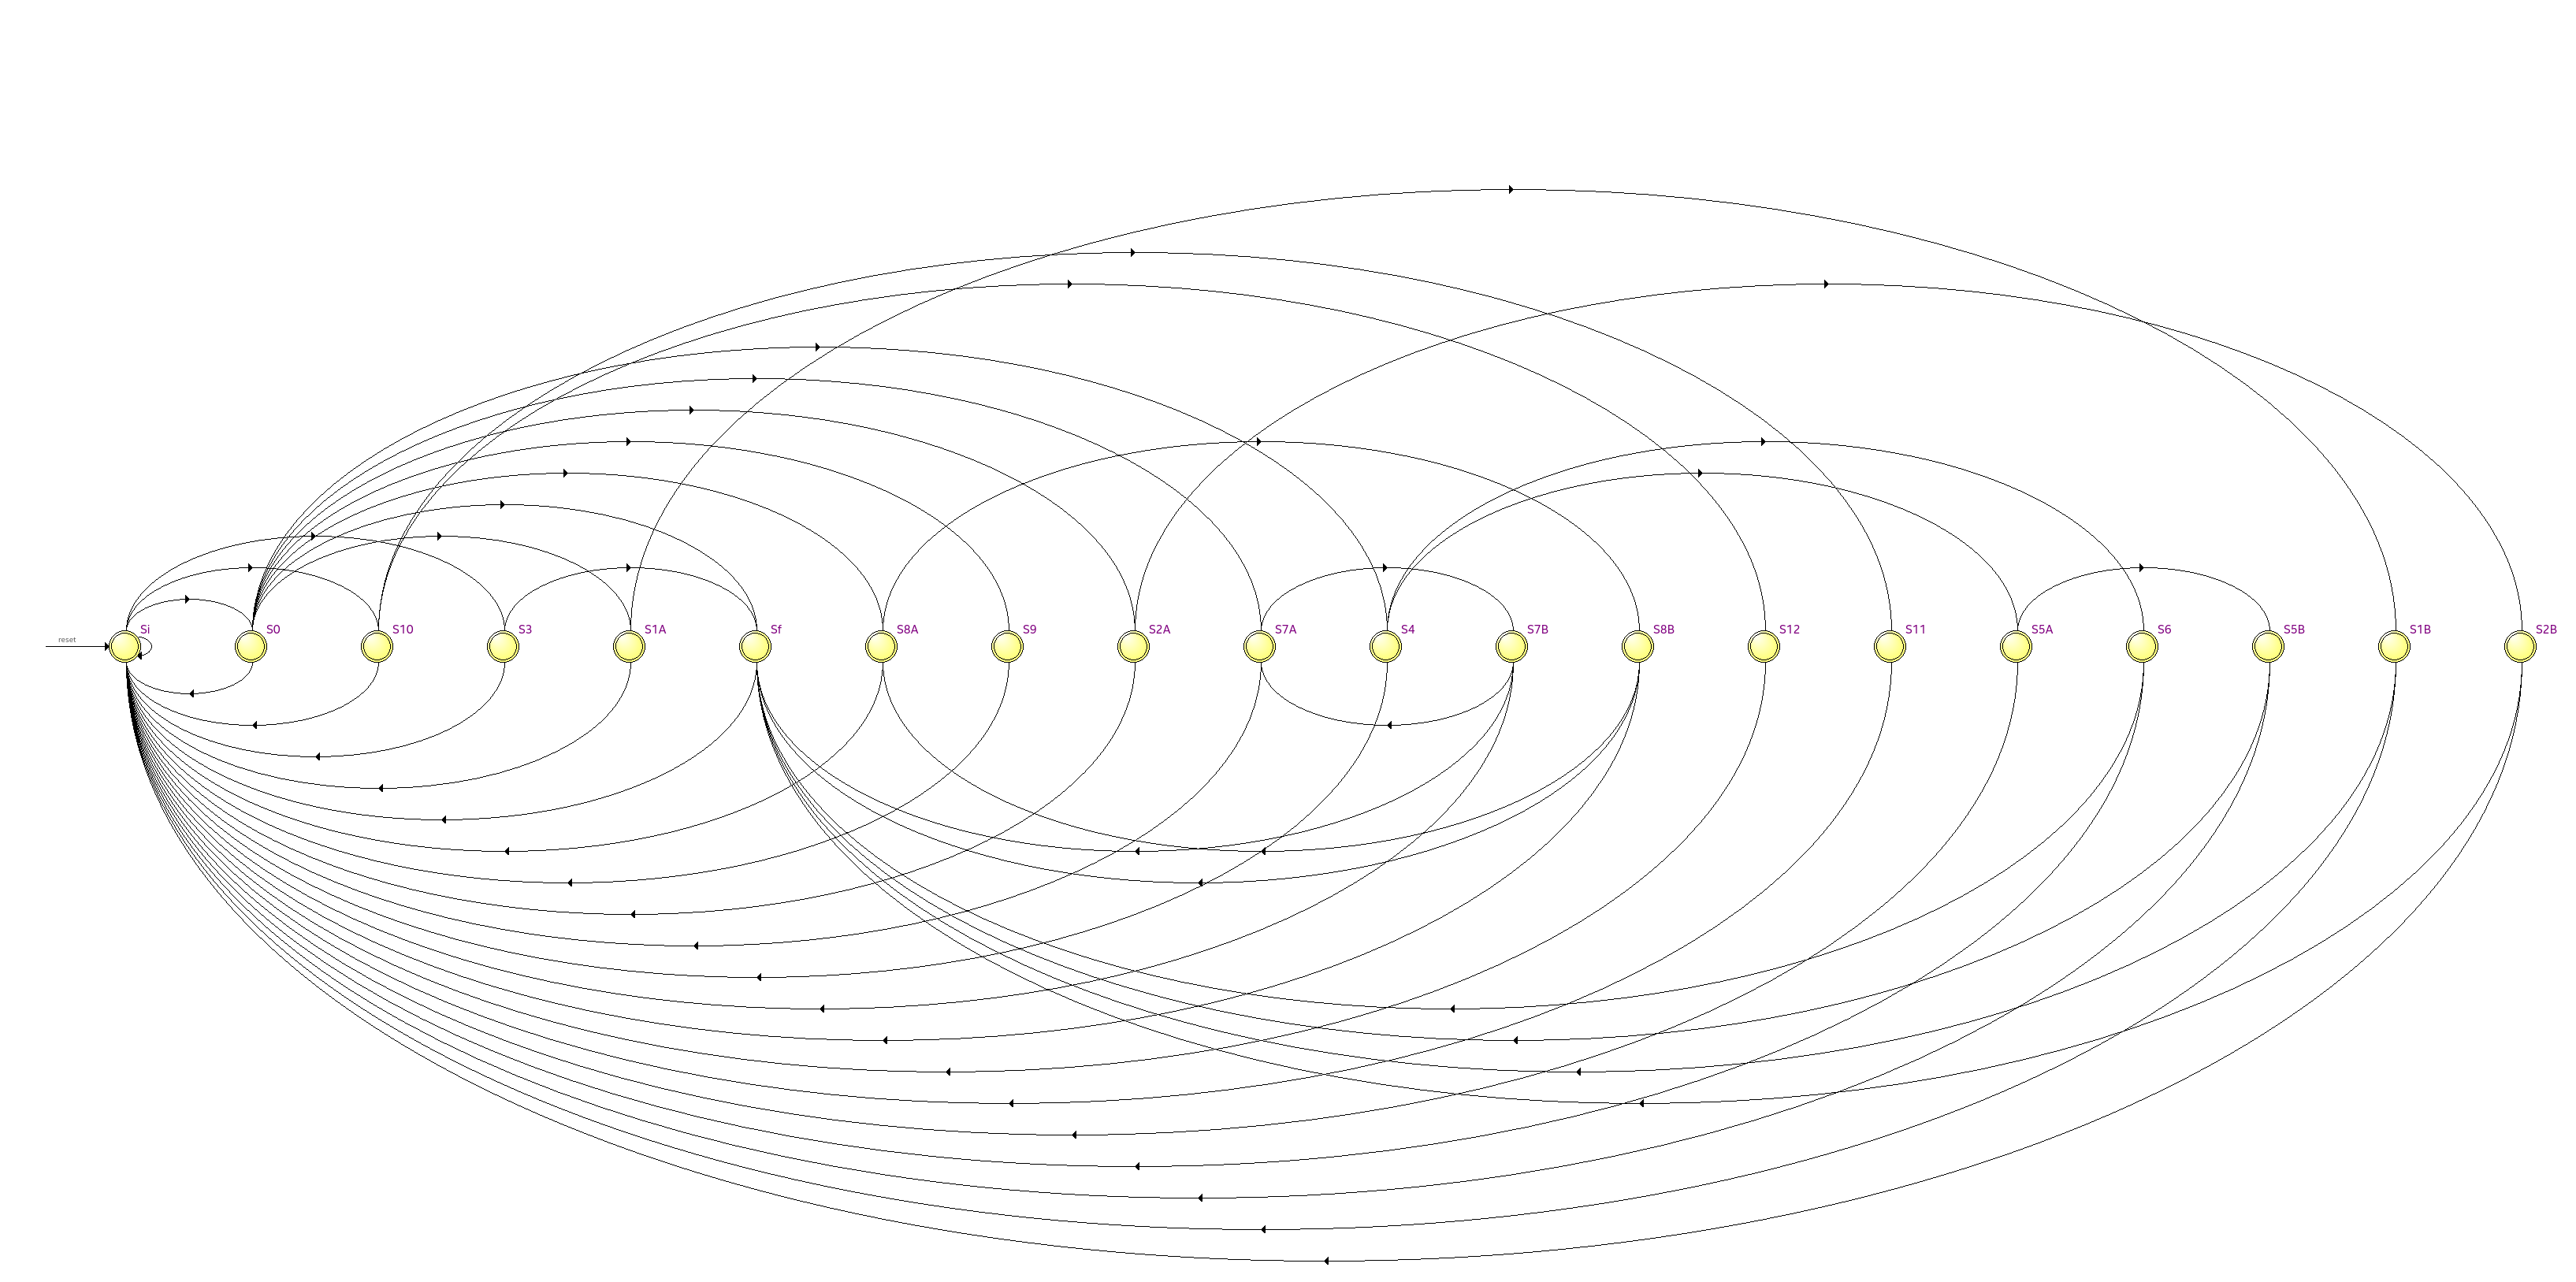
\includegraphics[scale=0.33]{FSM.png}
\end{sidewaysfigure}

\end{document}